%
% gradskala.tex -- Gradskala: elementar | elliptisch | hyperelliptisch
%
% Einordnung des Grades des Polynoms p(x) unter der Wurzel in
% \int R(x, sqrt(p(x))) dx: Grad 0,1,2 elementar, Grad 3,4 elliptisch,
% Grad >= 5 hyperelliptisch. Die Schwelle 2|3 ist die Hauptgrenze
% (dick, rot), die Schwelle 4|5 nur eine Einordnung (duenn, grau).
%
\documentclass[tikz]{standalone}
\usepackage{amsmath}
\usepackage{amssymb}
\usepackage{times}
\usepackage{txfonts}
\usetikzlibrary{decorations.pathreplacing}
\definecolor{darkred}{rgb}{0.8,0,0}
\definecolor{darkgreen}{rgb}{0,0.6,0}
\begin{document}
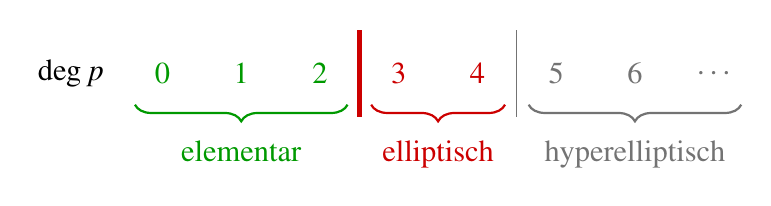
\begin{tikzpicture}[>=latex, thick, every node/.style={scale=1.1}]

% Zahlenreihe: Grad des Polynoms unter der Wurzel
\node[darkgreen]  at (0,0) {$0$};
\node[darkgreen]  at (1,0) {$1$};
\node[darkgreen]  at (2,0) {$2$};
\node[darkred]    at (3,0) {$3$};
\node[darkred]    at (4,0) {$4$};
\node[black!55]   at (5,0) {$5$};
\node[black!55]   at (6,0) {$6$};
\node[black!55]   at (7,0) {$\ldots$};

% Achsenlabel links
\node[anchor=east] at (-0.6,0) {$\deg p$};

% Gruppenklammern mit Beschriftung
\draw[decorate, decoration={brace, mirror, amplitude=6pt}, darkgreen]
	(-0.35,-0.4) -- (2.35,-0.4)
	node[midway, below=8pt, darkgreen] {elementar};
\draw[decorate, decoration={brace, mirror, amplitude=6pt}, darkred]
	(2.65,-0.4) -- (4.35,-0.4)
	node[midway, below=8pt, darkred] {elliptisch};
\draw[decorate, decoration={brace, mirror, amplitude=6pt}, black!55]
	(4.65,-0.4) -- (7.35,-0.4)
	node[midway, below=8pt, black!55] {hyperelliptisch};

% Trennlinien: Hauptgrenze 2|3 dick rot, Nebengrenze 4|5 duenn grau
\draw[darkred, line width=1.6pt] (2.5,-0.55) -- (2.5,0.55);
\draw[black!55, thin]            (4.5,-0.55) -- (4.5,0.55);

\end{tikzpicture}
\end{document}
